\let\negmedspace\undefined
\let\negthickspace\undefined
\documentclass[journal]{IEEEtran}
\usepackage[a5paper, margin=10mm, onecolumn]{geometry}
\usepackage{lmodern} % Ensure lmodern is loaded for pdflatex
\usepackage{tfrupee} % Include tfrupee package

\setlength{\headheight}{1cm} % Set the height of the header box
\setlength{\headsep}{0mm}     % Set the distance between the header box and the top of the text

\usepackage{gvv-book}
\usepackage{gvv}
\usepackage{cite}
\usepackage{amsmath,amssymb,amsfonts,amsthm}
\usepackage{algorithmic}
\usepackage{graphicx}
\usepackage{textcomp}
\usepackage{xcolor}
\usepackage{txfonts}
\usepackage{listings}
\usepackage{enumitem}
\usepackage{mathtools}
\usepackage{gensymb}
\usepackage{comment}
\usepackage[breaklinks=true]{hyperref}
\usepackage{tkz-euclide} 
\usepackage{listings}
\usepackage{gvv}                                        
\def\inputGnumericTable{}                                 
\usepackage[latin1]{inputenc}                                
\usepackage{color}                                            
\usepackage{array}                                            
\usepackage{longtable}                                       
\usepackage{calc}                                             
\usepackage{multirow}                                         
\usepackage{hhline}                                           
\usepackage{ifthen}                                           
\usepackage{lscape}
\begin{document}

\bibliographystyle{IEEEtran}
\vspace{3cm}

\title{6.5.3.6}
\author{EE24BTECH11016 - DHWANITH M DODDAHUNDI}
 \maketitle
% \newpage
% \bigskip
{\let\newpage\relax\maketitle}

\renewcommand{\thefigure}{\theenumi}
\renewcommand{\thetable}{\theenumi}
\setlength{\intextsep}{10pt} % Space between text and floats


\numberwithin{equation}{enumi}
\numberwithin{figure}{enumi}
\renewcommand{\thetable}{\theenumi}


\textbf{Question}:\\
Find the local minimum/maximum of the given function:\\
$f\brak{x} = \frac{x}{2} + \frac{2}{x}$
\\
\textbf{Solution: }\\
For the function,
\begin{align}
y\brak{x} &= \frac{x}{2} + \frac{2}{x} \\
    y\prime\brak{x} &= \frac{1}{2}-\frac{2}{x^{2}}\\
    y\prime\prime\brak{x} &= \frac{4}{x^{3}}
\end{align}
For critical points,
\begin{align}
    y\prime\brak{x} &= 0\\
    \implies   \frac{1}{2}-\frac{2}{x^{2}} &=0\\
    \implies    x^{2}=4 \\
    \implies    x &= -2,2
\end{align}
For, critical points to be local minimum or local maximum, it should follow the following:-
\begin{align}
    \text{Local Minimum:}\, y\prime\prime\brak{x}&\textgreater 0\\
    \text{Local Maximum:}\, y\prime\prime\brak{x} &\textless 0
\end{align}
For,$x=-2$ we get,
\begin{align}
    y\prime\prime\brak{-2} &= \frac{4}{\brak{-2}^{3}}\\
    y\prime\prime\brak{-2} &= -\frac{1}{2}\,\textless0
\end{align}
So, $x=-2$ is a point of local maxima.\\ \\
For, $x=2$ we get,
\begin{align}
    y\prime\prime\brak{2} &= \frac{4}{\brak{2}^{3}}\\
    y\prime\prime\brak{2} &= \frac{1}{2}\,\textgreater 0
\end{align}
So, $x=2$ is a point of local minima.\\
\textbf{Computational Solution:}\\
Finding the Local Maxima using Gradient Ascent we get,
\begin{align}
    x_{n+1} &= x_n + \alpha f\prime\brak{x_n}\\
    x_{n+1} &= x_n + \alpha\brak{\frac{1}{2}-\frac{2}{x^{2}} }
\end{align}
Finding the Local Minima using Gradient Decent we get,
\begin{align}
    x_{n+1} &= x_n - \alpha f\prime\brak{x_n}\\
    x_{n+1} &= x_n - \alpha\brak{\frac{1}{2}-\frac{2}{x^{2}} }
\end{align}
Taking the following conditions, we have
\begin{align}
    x_0 &= 0.5\\
    h &= 0.01\\
    \alpha &=0.1
\end{align}
After computing we get,
\begin{align}
    \text{Local maxima:}\, x&=1.999981868996581,\,f\brak{x} = 2.000000000082184\\
    \text{Local Minima:}\, x&=-2.0000188911077013,\,f\brak{x} = -2.0000000000892175
\end{align}

\begin{figure}[H]
    \centering
    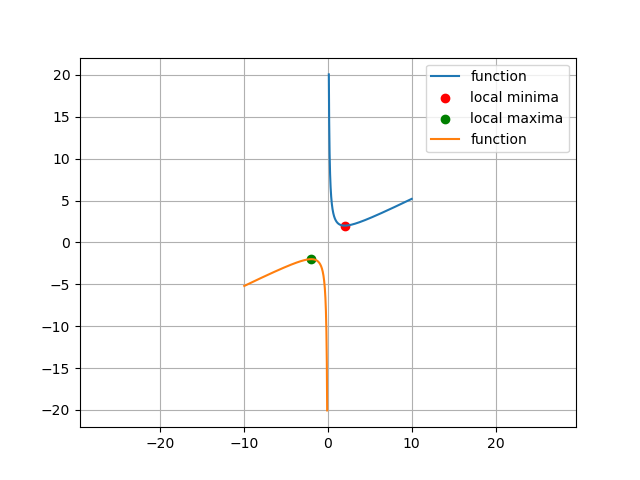
\includegraphics[width=\columnwidth]{figs/plot.png}
    \caption{Maxima and Minima points of the given function}
    \label{fig:Plot1}
    \end{figure}

\end{document}

